% !TEX TS-program = XeLaTeX

\documentclass[usenames, xcolor=dvipsnames]{beamer}
%% \documentclass[professionalfonts, xcolor=table, handout]{beamer}
%% \usepackage{pgfpages}
%% \pgfpagesuselayout{4 on 1}[a4paper,border shrink=5mm, landscape]
\usepackage{fontspec}
\usepackage{amsmath,amssymb}
\usepackage{pifont}% http://ctan.org/pkg/pifont
\usepackage{tikz}
\usetikzlibrary{positioning, matrix, arrows.meta, shapes.geometric, calc,
  decorations.pathmorphing, decorations.pathreplacing, fit, shapes.multipart}
\usepackage{mathabx}
\usepackage{mathtools}
\usepackage{mathpartir}
\usepackage{fancyvrb}
\usepackage{stmaryrd}
\usepackage[absolute,overlay]{textpos}
\usepackage[export]{adjustbox} % for subfigures
\usepackage[normalem]{ulem} % for strikeout
\usepackage{listings}

\lstdefinestyle{myTinyStyle}{
	%   language=Coq,
	basicstyle=\tiny,
	stepnumber=1,
	tabsize=2,
	numbers=none,
	numberstyle=\tiny,
	numbersep=5pt,
	showspaces=false,
	showstringspaces=false,
	language=C,
	morecomment=[l][{\color{OliveGreen}}]{//},
	sensitive=true,
	mathescape=true,
	escapechar=`,
	basicstyle=\tt,
	keywordstyle=\color{black},
	numbersep=5pt, boxpos=t
}

\lstset{style=myTinyStyle}

\definecolor{lightg}{RGB}{217,232,225}
\definecolor{darkg}{RGB}{6,81,42}
\definecolor{myred}{rgb}{0.0, 0.42, 0.24}
\colorlet{mypink}{myred!50!white}
\definecolor{mymaroon}{rgb}{0.86, 0.08, 0.24}

\defaultfontfeatures{Mapping=tex-text,Scale=MatchLowercase}
% \setmainfont{Libertinus Serif}
% \setsansfont{Libertinus Sans}
% \setmonofont{Menlo Regular}
\usetheme{Madrid}
\useoutertheme{infolines} % Alternatively: miniframes, infolines, split
\useinnertheme{circles}

% \setbeamertemplate{enumerate item}[default]
\usecolortheme[named=myred]{structure}
% \usecolortheme{spruce}
\usefonttheme{serif}
\setbeamerfont*{frametitle}{series=\bfseries}
\setbeamercolor{alerted text}{fg=mymaroon}
\setbeamertemplate{navigation symbols}{}
\setbeamercolor{emphC}{fg=myred}
% \setbeamercolor{block title}{bg = darkg, fg=white!80}
% \setbeamercolor{block body}{bg = lightg, fg=black}
\setbeamercolor{itemize item}{fg=black}
\setbeamercolor{description item}{fg=myred}

\newcommand{\sz}{\texttt{size}}
\newcommand{\ifty}{\texttt{inf}}
\newcommand{\scon}{\mathbin{\ast}}
\usepackage{scalerel}
\renewcommand{\bigstar}{\raisebox{-0.24em}{{\scaleobj{2.5}{\scon}}}}

\newcommand{\ocon}{%
  \mathbin{\mbox{$\mathrlap{\cup}\hspace*{.15em}
      \raisebox{.01em}[0ex][0ex]{$\scon$}$\hspace*{.07em}}}}
\newcommand{\medocon}{
  \raisebox{-0.3ex}{\resizebox{0.63em}{!}{$\scon$}} \hspace{-2.4ex} \bigcup}
\newcommand{\wand}{%
 \mathrel{\mbox{$\hspace*{-0.03em}\mathord{-}\hspace*{-0.66em}
  \mathord{-}\hspace*{-0.36em}\mathord{\scon}$\hspace*{-0.005em}}}}
\newcommand{\defeq}{\mathbin{\stackrel{\Delta}{=}}}
\newcommand{\emphd}[1]{{\bfseries #1}}
\newcommand{\emphr}[2]{\alert<#1>{#2}}
\newcommand{\bracket}[1]{[#1]}
\newcommand{\hide}[1]{}
\newcommand{\braces}[1]{\color{OliveGreen}\left\{\begin{array}{l@{}} \!\!\! #1 \end{array}\right\}}
\newcommand{\s}{11}

\makeatletter\let\frametextheight\beamer@frametextheight\makeatother
\newcommand\credit[1]{%
  \begin{textblock*}{\paperwidth}(0pt,\textheight)
    \raggedleft #1\hspace{.5em}
\end{textblock*}}
\newcommand{\pguards}[1]{\llbracket #1 \rrbracket}
\newcommand{\xmark}{\ding{55}}%
\newcommand{\cmark}{\ding{51}}%
\newcommand{\m}[1]{\ensuremath{\mathit{#1}}} % math font
\newcommand{\p}[1]{\ensuremath{\mathsf{#1}}} % predicate font
\newcommand{\bi}{\Leftrightarrow} % equivalence of expressions

\AtBeginSection[]
{
  \begin{frame}
    \frametitle{Outline}
    \tableofcontents[currentsection]
  \end{frame}
}

\setbeamertemplate{section in toc}{%
  \inserttocsectionnumber.~\inserttocsection}
\setbeamercolor{subsection in toc}{bg=white,fg=structure}
\setbeamertemplate{subsection in toc}{%
  \hspace{1.2em}{\rule[0.3ex]{3pt}{3pt}}~\inserttocsubsection\par}


\title[Verifying Dijkstra, Prim, Kruskal]{Functional Correctness of Dijkstra's, Prim's, \\ and Kruskal's Algorithms in C}
\author[]{\underline{Anshuman Mohan} \\ Leow Wei Xiang \\ Aquinas Hobor}
%\institute[NUS]{
\includegraphics[height=0.12\textwidth]{NUS_logo_full-horizontal.jpg}}
  \date[]{Cornell PLDG \\ \today}

\begin{document}
\begin{frame}[plain]
  \titlepage
\end{frame}

\begingroup
    \AtBeginSection[]{}
\section{CertiGraph: Motivation and Overview}
\endgroup

\begin{frame}{Refresher: Dijkstra, Prim, Kruskal}

{\centering
\begin{adjustbox}{scale=0.9}
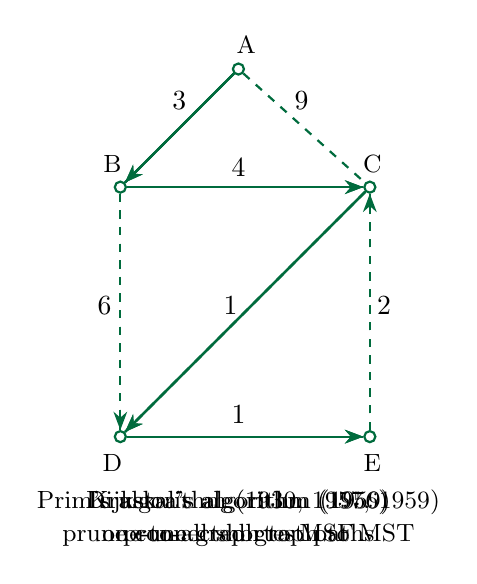
\begin{tikzpicture}
[vad/.style={rectangle, fill=black, inner sep=0pt, minimum size=4pt},
 inf/.style={circle, draw=myred, thick, inner sep=0pt, minimum size=4pt},
 inv/.style={circle, fill=myred, draw=myred, thick, inner sep=0pt, minimum size=4pt},
 ->/.style={thick, arrows={-Stealth}},
 every text node part/.style={align=center}]
 
% static vertices and their labels
\node at (1.6, 1.8) {\small A};
\node at (-0.1, 0.3) {\small B};
\node at (3.2, 0.3) {\small C};
\node at (-0.1, -3.5) {\small D}; 
\node at (3.2, -3.5) {\small E}; 
\node[inf] (A) at (1.5,1.5) {};  
\node[inf] (B) at (0,0) {};
\node[inf] (C) [right = 3 of B] {};
\node[inf] (D) [below = 3 of B] {};
\node[inf] (E) [below = 3 of C] {};

% names
  \uncover<1,2>{\node at (1.5,-4.2) {\small Dijkstra's algorithm (1959) \\ 
  \small one-to-all shortest paths};}
  \uncover<3,4>{\node at (1.5,-4.2) {\small Prim's algorithm (1930, 1957, 1959) \\
  \small prune connected graph to MST};}
  \uncover<5,6>{\node at (1.5,-4.2) {\small Kruskal's algorithm (1956) \\ 
  \small prune graph to MSF};}

%edge labels 
\node at (.75,1.1) {3};
\node at (1.5,0.25) {4};
\node at (1.5,-2.89) {1};
\uncover<1-3>{\node at (-0.2,-1.5) {6};
			\node at (3.35,-1.5) {2};}
\uncover<1-4>{\node at (1.4,-1.5) {1};}
\uncover<3,5>{\node at (2.3,1.1) {9};}

%edges for Dijkstra
\uncover<1,2>{
  \draw [->, dashed, myred] (A) -- (B);
  \draw [->, dashed, myred] (B) -- (C);
  \draw [->, dashed, myred] (D) -- (E);  
  \draw [->, dashed, myred] (B) -- (D);
  \draw [->, dashed, myred] (E) -- (C);
  \draw [->, dashed, myred] (C) -- (D);
 }
\uncover<2>{
  \draw [->, myred] (A) -- (B);
  \draw [->, myred] (B) -- (C);
  \draw [->, myred] (D) -- (E);  
  \draw [->, myred] (C) -- (D);
 }
  
 %undirected
 \uncover<3,5>{
  \draw [thick, dashed, myred] (B) -- (A);
  \draw [thick, dashed, myred] (C) -- (B);
  \draw [thick, dashed, myred] (E) -- (D);}
 \uncover<4,6>{
  \draw [thick, myred] (B) -- (A);
  \draw [thick, myred] (C) -- (B);
  \draw [thick, myred] (E) -- (D);}

\uncover<3>{
 \draw [thick, dashed, myred] (C) -- (D);
 }
 \uncover<4>{
 \draw [thick, myred] (C) -- (D);
 }
 \uncover<3>{
  \draw [thick, dashed, myred] (B) -- (D);
  \draw [thick, dashed, myred] (E) -- (C);
}
 \uncover<3,5>{
 \draw [thick, dashed, myred] (A) -- (C);
 }
\end{tikzpicture}
\end{adjustbox}

}% end centering
\end{frame}

\begin{frame}{Motivation: a precondition for Dijkstra}

In a graph with \texttt{size} vertices, \\
the longest optimal path has \texttt{size-1} links \\
\uncover<2->{so an edge-cost is, at most, $\lfloor\texttt{MAX/(size-1)}\rfloor$}

\bigskip \uncover<3->{
Consider a $4$-bit machine and unsigned integers \\
\texttt{MAX} = 15, \texttt{size} = 3, so every edge-cost $\le 7$.}

\bigskip

{\centering
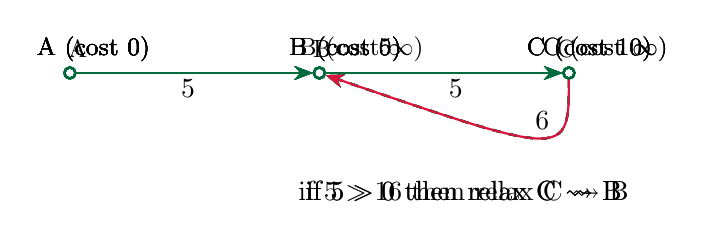
\begin{tikzpicture}
[inf/.style={circle, draw=myred, thick, inner sep=0pt, minimum size=4pt},
 ->/.style={thick, arrows={-Stealth}}]

\uncover<3->{
  \node at (1.5,-0.2) {5};
  \node at (4.9,-0.2) {5};
  \node at (6,-0.6) {6};
  }

\uncover<1,2>{
\node at (0.1, 0.3) {\small A};
\node at (3.2, 0.3) {\small B};
\node at (6.3, 0.3) {\small C}; 
  \node[inf] (A) at (0,0) {};
  \node[inf] (B) [right = 3 of A] {};
  \node[inf] (C) [right = 3 of B] {};
  \draw [->, dashed, myred] (A) -- (B);
  \draw [->, dashed, myred] (B) -- (C);}


\uncover<3>{
\node at (0.3, 0.3) {\small A (cost 0)};
\node at (3.7, 0.3) {\small B (cost $\infty$)};
\node at (6.8, 0.3) {\small C (cost $\infty$)}; 
  \node[inf] (A) at (0,0) {};
  \node[inf] (B) [right = 3 of A] {};
  \node[inf] (C) [right = 3 of B] {};
  \draw [->, dashed, myred] (A) -- (B);
  \draw [->, dashed, myred] (B) -- (C);
  \draw [->, dashed, myred] (C.south) .. controls ++(0, -1) .. (B);}
 
\uncover<4>{
\node at (0.3, 0.3) {\small A (cost 0)};
\node at (3.5, 0.3) {\small B (cost 5)};
\node at (6.8, 0.3) {\small C (cost $\infty$)};  
  \node[inf] (A) at (0,0) {};
  \node[inf] (B) [right = 3 of A] {};
  \node[inf] (C) [right = 3 of B] {};
  \draw [->, myred] (A) -- (B);
  \draw [->, dashed, myred] (B) -- (C);
  \draw [->, dashed, myred] (C.south) .. controls ++(0, -1) .. (B);
  }

\uncover<5>{ 
\node at (0.3, 0.3) {\small A (cost 0)};
\node at (3.5, 0.3) {\small B (cost 5)};
\node at (6.6, 0.3) {\small C (cost 10)};  
  \node[inf] (A) at (0,0) {};
  \node[inf] (B) [right = 3 of A] {};
  \node[inf] (C) [right = 3 of B] {};
  \draw [->, myred] (A) -- (B);
  \draw [->, myred] (B) -- (C);
  \draw [->, dashed, myred] (C.south) .. controls ++(0, -1) .. (B);
}

\uncover<6>{ 
\node at (0.3, 0.3) {\small A (cost 0)};
\node at (3.5, 0.3) {\small B (cost 5)};
\node at (6.6, 0.3) {\small C (cost 10)};  
\node at (5, -1.5) {if $5 > 16$ then relax C $\leadsto$ B};
  \node[inf] (A) at (0,0) {};
  \node[inf] (B) [right = 3 of A] {};
  \node[inf] (C) [right = 3 of B] {};
  \draw [->, myred] (A) -- (B);
  \draw [->, myred] (B) -- (C);
  \draw [->, dashed, myred] (C.south) .. controls ++(0, -1) .. (B);
}

\uncover<7>{ 
\node at (0.3, 0.3) {\small A (cost 0)};
\node at (3.5, 0.3) {\small B (cost 5)};
\node at (6.6, 0.3) {\small C (cost 10)};  
\node at (5, -1.5) {if $5 > \alert{0}$ then relax C $\leadsto$ B};
  \node[inf] (A) at (0,0) {};
  \node[inf] (B) [right = 3 of A] {};
  \node[inf] (C) [right = 3 of B] {};
  \draw [->, myred] (A) -- (B);
  \draw [->, myred] (B) -- (C);
  \draw [->, dashed, myred] (C.south) .. controls ++(0, -1) .. (B);
}

\uncover<8->{ 
\node at (0.3, 0.3) {\small A (cost 0)};
\node at (3.5, 0.3) {\small B (cost \alert{0})};
\node at (6.6, 0.3) {\small C (cost 10)}; 
\node at (5, -1.5) {if $5 > 0$ then \alert{relax C $\leadsto$ B}};
  \node[inf] (A) at (0,0) {};
  \node[inf] (B) [right = 3 of A] {};
  \node[inf] (C) [right = 3 of B] {};
  \draw [->, myred] (A) -- (B);
  \draw [->, myred] (B) -- (C);
  \draw [->, mymaroon] (C.south) .. controls ++(0, -1) .. (B);
}

\end{tikzpicture}

}
\bigskip
\uncover<9->{
Must allow room for the probe edge 
\includegraphics[scale=.08]{nye} \\ }
\uncover<10>{so an edge-cost is, at most, \alert{$\lfloor\texttt{MAX/size}\rfloor$}}

\end{frame}

\begin{frame}{Motivation: A precondition for Dijkstra}

There are many ways to fix this!
\\ \hspace{1em} Refactor troublesome addition as subtraction
\\ \hspace{1em} Coerce to \texttt{long}
\\ \hspace{1em} Work in \texttt{float}, which has $\infty^{+}$
\\ \hspace{1em} Never look back into optimized part

\bigskip

\pause Sadly, intuition supports our misstep \\
and bugs such as this one are often overlooked

\end{frame}

\begin{frame}{CertiGraph: problem scope}

\includegraphics[scale=0.09]{vst_logo}
\hspace{2em} 
\includegraphics[scale=0.12]{compcert_logo}
\hspace{2em} 
\includegraphics[scale=0.2]{paper_screen}

\bigskip
VST + CompCert + \underline{CertiGraph}

\bigskip
\hspace{1em}Verify executable code
\\\hspace{1em}against realistic specifications
\\\hspace{1em}expressed with mathematical graphs

\end{frame}

\begin{frame}{CertiGraph: workflow}
    
\begin{tikzpicture}[remember picture,overlay, on grid,
      ourlib/.style={rounded corners=4pt, line width=0.8pt},
      cmd/.style={rectangle, fill=yellow!50!white, draw=black, rounded corners=4pt},
      file/.style={rounded corners=2pt, line width=1pt, fill=yellow!50!white},
      ->/.style={-Stealth, line width=1pt}]
    \path
    coordinate (nw) at ($(current page.north west) + (0.25, -1.5)$)
    coordinate (ne) at ($(current page.north east) + (-0.25, -1.5)$)
    coordinate (sw) at ($(current page.south west) + (0.25, 0.5)$)
    coordinate (se) at ($(current page.south east) + (-0.25, 0.5)$)
    coordinate (cright) at ($(current page.south west) + (2.85, 0.5)$)
    coordinate (asmleft) at ($(current page.south east) + (-2.85, 0.5)$)
    coordinate (coqleft) at ($(current page.south west)!.5!(current page.south east) +
    (-0.5, 0.5)$)
    coordinate (coqright) at ($(current page.south west)!.5!(current page.south east) +
    (0.5, 0.5)$);
    \draw [ourlib, fill=green!20!white] (nw) rectangle ($(sw) + (0.8, 0)$);
    \node at ($(nw)!.5!(sw) + (0.4, 0)$)
          {\rotatebox{-90}{\textsf{Mathematical Graph Library}}};
    \draw [ourlib, fill=red!20!white] (ne) rectangle ($(se) + (-0.8, 0)$);
    \node at ($(ne)!.5!(se) + (-0.4, 0)$)
          {\rotatebox{-90}{\textsf{Verified Software Toolchain (VST)}}};
    \draw [ourlib, fill=green!20!white] ($(nw) + (1.6, 0)$) rectangle
    ($(ne) + (-1.6, -0.8)$);
    \node at ($(nw)!.5!(ne) + (0, -0.4)$) {\textsf{Spatial Graph Library}};

    \draw [ourlib, fill=green!20!white] ($(nw) + (1.6, -1.6)$) -- ++(0, -0.8) --
    ++(1.6, 0) -- ++(0, -0.8) -- ++(-1.6, 0) -- ++(0, -0.8) -- ++(3.6, 0) --
    ++(0, 0.8) -- ++(-1.6, 0) -- ++(0, 0.8) -- ++(2, 0) -- ++(0, -0.5) -- ++(-1.6, 0)
    -- ++(0, -1.4) -- ++(3.6, 0) -- ++(0, 1.4) -- ++(-1.6, 0) -- ++(0, 0.5) -- ++(2, 0)
    -- ++(0, -0.8) -- ++(-1.6, 0) -- ++(0, -0.8) -- ++(4.2, 0) -- ++(0, 0.8) --
    ++(-1.6, 0) -- ++(0, 0.8) -- ($(ne) + (-1.6, -2.4)$) -- ++(0, 0.8) -- cycle;
    \node at ($(nw)!.5!(ne) + (0, -2)$)
          {\textsf{Verification of a Graph-Manipulating Function}};
    \draw [ourlib, fill=red!20!white] ($(sw) + (1.6, 0)$) -- ++(0, 0.8) --
    ($(cright) + (0.6, 0.8)$) -- ++(0, 1.8) -- ($(coqleft) + (-0.6, 2.6)$) --
    ++(0, -1.8) -- ($(coqright) + (0.6, 0.8)$) -- ++(0, 1.8) --
    ($(asmleft) + (-0.6, 2.6)$) -- ++(0, -1.8) -- ($(se) + (-1.6, 0.8)$) --
    ++(0, -0.8) -- cycle;
    \node at ($(sw)!.5!(se) + (0, 0.4)$) {\textsf{The CompCert Project}};
    \node (P0) at ($(nw) + (2.2, -3.6)$) {$\{P_0\}$};
    \node (C1) [cmd, right=1.2 of P0] {$C_1$};
    \node (P1) [right=2.4 of P0] {$\{P_1\}$};
    \node (P2) [right=2.4 of P1] {$\{P_2\}$};
    \node (P3) [right=2.8 of P2] {$\{...P_n\}$};
    \node (C2) [cmd, right=2.4 of C1] {$C_2$};
    \node (C3) [cmd, right=2.8 of C2] {$...C_n$};
    \draw [file] ($(sw)!.5!(se) + (-0.5, 1.2)$) -- ++(1, 0) -- ++ (0, 1.1) --
    +(-0.3, 0.3) -- +(-1, 0.3) -- cycle ++(1, 1.1) -- ++(-0.3, 0) -- ++(0, 0.3);
    \node at ($(sw)!.5!(se) + (0, 1.9)$) {\textsf{Coq}};
    \draw [file] ($(sw) + (1.6, 1.2)$) -- ++(1, 0) -- ++ (0, 1.1) --
    +(-0.3, 0.3) -- +(-1, 0.3) -- cycle ++(1, 1.1) -- ++(-0.3, 0) -- ++(0, 0.3);
    \node at ($(sw) + (2.1, 1.9)$) {\textsf{C}};
    \draw [file] ($(se) + (-2.6, 1.2)$) -- ++(1, 0) -- ++ (0, 1.1) --
    +(-0.3, 0.3) -- +(-1, 0.3) -- cycle ++(1, 1.1) -- ++(-0.3, 0) -- ++(0, 0.3);
    \node at ($(se) + (-2.1, 1.9)$) {\textsf{Asm}};
    \draw [->, dashed] ($(sw)!.5!(se) + (-0.3, 2.6)$) .. controls ++(-0.3, 0.5) and
    ($(C1.south) + (0.3, -1)$) .. (C1.south);
    \draw [->, dashed] ($(sw)!.5!(se) + (-0.2, 2.6)$) -- (C2.south);
    \draw [->, dashed] ($(sw)!.5!(se) + (-0.1, 2.6)$) .. controls ++(0.3, 0.5) and
    ($(C3.south) + (-0.3, -1)$) .. (C3.south);
    \node at ($(cright)!.5!(coqleft) + (0, 1.9)$) {\begin{tabular}{c} \textsf{Parser,}
        \\ \textsf{Simplifier} \end{tabular}};
    \node at ($(coqright)!.5!(asmleft) + (0, 1.9)$) {\begin{tabular}{c}
        \textsf{Verified} \\ \textsf{Compiler} \end{tabular}};
    \draw [->] ($(cright) + (0, 1.9)$) -- ++(0.6, 0);
    \draw [->] ($(coqleft) + (-0.6, 1.9)$) -- ++(0.6, 0);
    \draw [->] ($(coqright) + (0, 1.9)$) -- ++(0.6, 0);
    \draw [->] ($(asmleft) + (-0.6, 1.9)$) -- ++(0.6, 0);

    %% left interface
    \draw [line width=2pt] ($(nw) + (1.8, -0.4)$) -- +(-0.4, 0) +(-0.7, 0) --
    +(-1.2, 0) +(-0.6, -0.2) arc [start angle=-90, end angle=90, radius=0.2];
    \fill ($(nw) + (1.2, -0.4)$) circle [radius=0.1];
    \draw [line width=2pt] ($(nw) + (1.8, -2)$) -- +(-0.4, 0) +(-0.7, 0) --
    +(-1.2, 0) +(-0.6, -0.2) arc [start angle=-90, end angle=90, radius=0.2];
    \fill ($(nw) + (1.2, -2)$) circle [radius=0.1];

    %% right interface
    \draw [line width=2pt] ($(ne) + (-1.8, -2)$) -- +(0.4, 0) +(0.7, 0) --
    +(1.2, 0) +(0.6, 0.2) arc [start angle=90, end angle=270, radius=0.2];
    \fill ($(ne) + (-1.2, -2)$) circle [radius=0.1];
    \draw [line width=2pt] ($(se) + (-0.6, 0.4)$) -- +(-0.4, 0) +(-0.7, 0) --
    +(-1.2, 0) +(-0.6, -0.2) arc [start angle=-90, end angle=90, radius=0.2];
    \fill ($(se) + (-1.2, 0.4)$) circle [radius=0.1]; 
    
    %% up interface
    \draw [line width=2pt] ($(ne)!.5!(nw) + (2, -1.8)$) -- +(0, 0.4) +(0, 0.7) --
    +(0, 1.2) +(0.2, 0.6) arc [start angle=0, end angle=-180, radius=0.2];
    \fill ($(ne)!.5!(nw) + (2, -1.2)$) circle [radius=0.1];
  \end{tikzpicture}
\end{frame}

\begin{frame}{CertiGraph: pure math graphs}
  \begin{align*}
\Big(\hspace{0.5em}\mathcal{V}& \texttt{: Type}, \\
\mathcal{E}& \texttt{: Type}, \\
\texttt{vvalid}& \texttt{: }\mathcal{V} \rightarrow \texttt{Prop}, \\ 
\texttt{evalid}& \texttt{: }\mathcal{E} \rightarrow \texttt{Prop}, \\
\texttt{src}& \texttt{: }\mathcal{E} \rightarrow \mathcal{V}, \\
\texttt{dst}& \texttt{: }\mathcal{E} \rightarrow \mathcal{V}, \\
\texttt{vlabel}& \texttt{: }\mathcal{V} \rightarrow \mathcal{L_V}, \\
\texttt{elabel}& \texttt{: }\mathcal{E} \rightarrow \mathcal{L_E}, \\
\texttt{sound}&\texttt{: Type} \hspace{0.5em} \Big) 
\end{align*}

\end{frame}

\begin{frame}
\frametitle{Outline}
\tableofcontents
\end{frame}

\section{Mathematical Adjacency Matrices}

\begin{frame}{Refresher: adjacency matrices}

\begin{minipage}{0.45\textwidth}
{\centering
\begin{adjustbox}{scale=0.9}
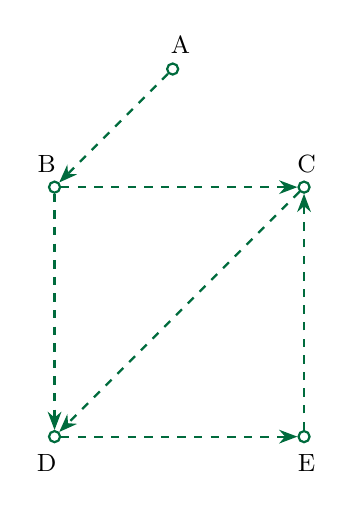
\begin{tikzpicture}
[vad/.style={rectangle, fill=black, inner sep=0pt, minimum size=4pt},
 inf/.style={circle, draw=myred, thick, inner sep=0pt, minimum size=4pt},
 inv/.style={circle, fill=myred, draw=myred, thick, inner sep=0pt, minimum size=4pt},
 ->/.style={thick, arrows={-Stealth}},
 every text node part/.style={align=center}]
 
% static vertices and their labels
\node at (1.6, 1.8) {\small A};
\node at (-0.1, 0.3) {\small B};
\node at (3.2, 0.3) {\small C};
\node at (-0.1, -3.5) {\small D}; 
\node at (3.2, -3.5) {\small E}; 
\node[inf] (A) at (1.5,1.5) {};  
\node[inf] (B) at (0,0) {};
\node[inf] (C) [right = 3 of B] {};
\node[inf] (D) [below = 3 of B] {};
\node[inf] (E) [below = 3 of C] {};

  \draw [->, dashed, myred] (A) -- (B);
  \draw [->, dashed, myred] (B) -- (C);
  \draw [->, dashed, myred] (D) -- (E);  
  \draw [->, dashed, myred] (B) -- (D);
  \draw [->, dashed, myred] (E) -- (C);
  \draw [->, dashed, myred] (C) -- (D);
 
\end{tikzpicture}
\end{adjustbox}

}
\end{minipage} \begin{minipage}{0.45\textwidth}
{\centering
\begin{adjustbox}{scale=0.9}
\tikz\draw grid(5,5)foreach[count=~]\l in 
{  , A, B, C, D, E,
 A, 0, 1, 0, 0, 0,
 B, 0, 0, 1, 1, 0,
 C, 0, 0, 0, 1, 0,
 D, 0, 0, 0, 0, 1, 
 E, 0, 0, 1, 0, 0}
{({-.5+mod(~-1,6},{5.5-div(~-1,6})node{\l}};

\end{adjustbox}

}
\end{minipage}

\vspace{0.9em}
\centering 0 means absence, 1 means presence

\end{frame}

\begin{frame}{Issue with edge-labeled adjacency matrices}
\begin{minipage}{0.45\textwidth}
{\centering
\begin{adjustbox}{scale=0.9}
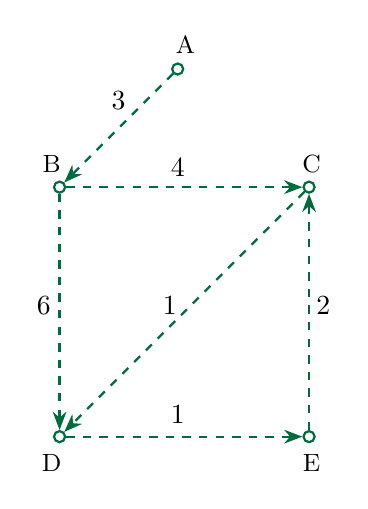
\begin{tikzpicture}
[vad/.style={rectangle, fill=black, inner sep=0pt, minimum size=4pt},
 inf/.style={circle, draw=myred, thick, inner sep=0pt, minimum size=4pt},
 inv/.style={circle, fill=myred, draw=myred, thick, inner sep=0pt, minimum size=4pt},
 ->/.style={thick, arrows={-Stealth}},
 every text node part/.style={align=center}]
 
% static vertices and their labels
\node at (1.6, 1.8) {\small A};
\node at (-0.1, 0.3) {\small B};
\node at (3.2, 0.3) {\small C};
\node at (-0.1, -3.5) {\small D}; 
\node at (3.2, -3.5) {\small E}; 
\node[inf] (A) at (1.5,1.5) {};  
\node[inf] (B) at (0,0) {};
\node[inf] (C) [right = 3 of B] {};
\node[inf] (D) [below = 3 of B] {};
\node[inf] (E) [below = 3 of C] {};

\node at (.75,1.1) {3};
\node at (1.5,0.25) {4};
\node at (1.5,-2.89) {1};
\node at (-0.2,-1.5) {6};
\node at (3.35,-1.5) {2};
\node at (1.4,-1.5) {1};

  \draw [->, dashed, myred] (A) -- (B);
  \draw [->, dashed, myred] (B) -- (C);
  \draw [->, dashed, myred] (D) -- (E);  
  \draw [->, dashed, myred] (B) -- (D);
  \draw [->, dashed, myred] (E) -- (C);
  \draw [->, dashed, myred] (C) -- (D);
 
\end{tikzpicture}
\end{adjustbox}

}
\end{minipage} \begin{minipage}{0.45\textwidth}
{\centering
\begin{adjustbox}{scale=0.9}
\tikz\draw grid(5,5)foreach[count=~]\l in 
{  , A, B, C, D, E,
 A, ?, 3, ?, ?, ?,
 B, ?, ?, 4, 6, ?,
 C, ?, ?, ?, 1, ?,
 D, ?, ?, ?, ?, 1, 
 E, ?, ?, 2, ?, ?}
{({-.5+mod(~-1,6},{5.5-div(~-1,6})node{\l}};
\end{adjustbox}

}

\end{minipage}

\vspace{0.9em}
\uncover<2>{\centering Inadvertently created a strongly-connected graph!}

\end{frame}

\begin{frame}{Supporting edge-labeled adjacency matrices}
\begin{minipage}{0.45\textwidth}
{\centering
\begin{adjustbox}{scale=0.9}
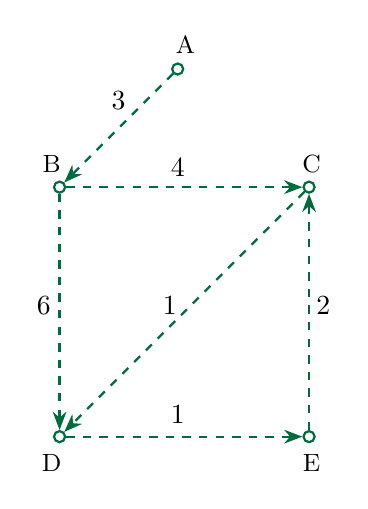
\begin{tikzpicture}
[vad/.style={rectangle, fill=black, inner sep=0pt, minimum size=4pt},
 inf/.style={circle, draw=myred, thick, inner sep=0pt, minimum size=4pt},
 inv/.style={circle, fill=myred, draw=myred, thick, inner sep=0pt, minimum size=4pt},
 ->/.style={thick, arrows={-Stealth}},
 every text node part/.style={align=center}]
 
% static vertices and their labels
\node at (1.6, 1.8) {\small A};
\node at (-0.1, 0.3) {\small B};
\node at (3.2, 0.3) {\small C};
\node at (-0.1, -3.5) {\small D}; 
\node at (3.2, -3.5) {\small E}; 
\node[inf] (A) at (1.5,1.5) {};  
\node[inf] (B) at (0,0) {};
\node[inf] (C) [right = 3 of B] {};
\node[inf] (D) [below = 3 of B] {};
\node[inf] (E) [below = 3 of C] {};

\node at (.75,1.1) {3};
\node at (1.5,0.25) {4};
\node at (1.5,-2.89) {1};
\node at (-0.2,-1.5) {6};
\node at (3.35,-1.5) {2};
\node at (1.4,-1.5) {1};

  \draw [->, dashed, myred] (A) -- (B);
  \draw [->, dashed, myred] (B) -- (C);
  \draw [->, dashed, myred] (D) -- (E);  
  \draw [->, dashed, myred] (B) -- (D);
  \draw [->, dashed, myred] (E) -- (C);
  \draw [->, dashed, myred] (C) -- (D);
 
\end{tikzpicture}
\end{adjustbox}

}
\end{minipage} \begin{minipage}{0.45\textwidth}
{\centering
\begin{adjustbox}{scale=0.9}
\tikz\draw grid(5,5)foreach[count=~]\l in 
{  , A, B, C, D, E,
 A, $\infty$, 3, $\infty$, $\infty$, $\infty$,
 B, $\infty$, $\infty$, 4, 6, $\infty$,
 C, $\infty$, $\infty$, $\infty$, 1, $\infty$,
 D, $\infty$, $\infty$, $\infty$, $\infty$, 1, 
 E, $\infty$, $\infty$, 2, $\infty$, $\infty$}
{({-.5+mod(~-1,6},{5.5-div(~-1,6})node{\l}};
\end{adjustbox}

}

\end{minipage}

\vspace{0.9em}
\uncover<2>{\centering Precondition: $\exists \infty.~$no bona-fide edge has cost $\infty$}
\end{frame}


\begin{frame}{Constraining a representable graph}
What graphs are representable as edge-labeled adjacency matrices? 

\bigskip 
\uncover<2->{
\vspace{-2em}
\begin{align*}
\Big(\hspace{0.5em}\mathcal{\alert<3>V}&\defeq\mathbb{\alert<3>Z}, \\
\mathcal{\alert<4>E}&\defeq\alert<4>{\mathcal{V} \times \mathcal{V}}, \\
\texttt{vvalid}&\defeq\ldots, \\ 
\texttt{evalid}&\defeq\ldots, \\
\texttt{\alert<5>{src}}&\defeq\m{\alert<5>{fst}}, \hspace{0.5em}\texttt{\alert<5>{dst}}\defeq\m{\alert<5>{snd}}, \\
\texttt{vlabel}&\defeq\ldots, \\
\texttt{elabel}&\defeq\ldots, \\
\alert<6>{\texttt{sound}}&\defeq\alert<6>{\texttt{SoundAdjMat size inf}}\hspace{0.5em}\Big) 
\end{align*}
}
\end{frame}

\begin{frame}[fragile]{A unified, reusable soundness condition}

\begin{lstlisting}
Class SoundAdjMat size inf g := {
  sr: 0 $<$ size $\le$ MAX;
  ir: MIN $\le$ inf $\le$ MAX; 
  vm: $\forall$v, vvalid g v $\leftrightarrow$ 0 $\le$ v $<$ size;
  em: $\forall$e, evalid g e $\leftrightarrow$ (MIN $\le$ elabel g e $\le$ MAX $\wedge$ 
                         elabel g e $\neq$ inf);
  iew: $\forall$e, $\neg$evalid g e $\leftrightarrow$ elabel g e = inf
}.
\end{lstlisting}

\pause \bigskip

Need more?
\begin{lstlisting}
Class SoundDijk size inf g := {
  sadjmat: SoundAdjMat size inf g;
  further: /* restrictions */
}.
\end{lstlisting}

\end{frame}


\section{Spatial Representations in Separation Logic}

\begin{frame}[fragile]{Laying out graphs in memory}
We support three flavors of adjacency matrix: \\
\hspace{1em}stack-allocated 2D~array \texttt{int~graph[size][size]} \\
\hspace{1em}stack-allocated 1D~array \texttt{int~graph[size$\times$size]} \\
\hspace{1em}heap-allocated 2D~array \texttt{int~**graph}

\bigskip

\uncover<2-3>{

\begin{minipage}{0.2\textwidth}
{\centering
\begin{adjustbox}{scale=0.5}
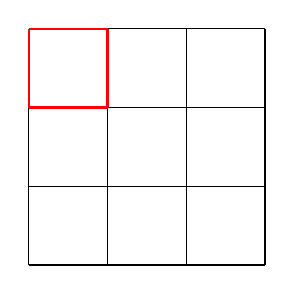
\begin{tikzpicture}
\draw grid(3,3);
\uncover<3>{\draw[red, thick, yshift=2cm] grid(1,1);}
\end{tikzpicture}
\end{adjustbox}

}
\end{minipage} \begin{minipage}{0.45\textwidth}
{\centering
\begin{adjustbox}{scale=0.5}

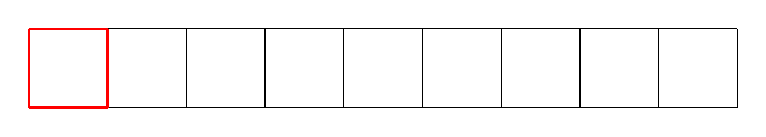
\begin{tikzpicture}
\draw grid(9,1);
\uncover<3>{\draw[red, thick] grid(1,1);}

\end{tikzpicture}
\end{adjustbox}

}
\end{minipage}\begin{minipage}{0.25\textwidth}
{\centering
\begin{adjustbox}{scale=0.5}
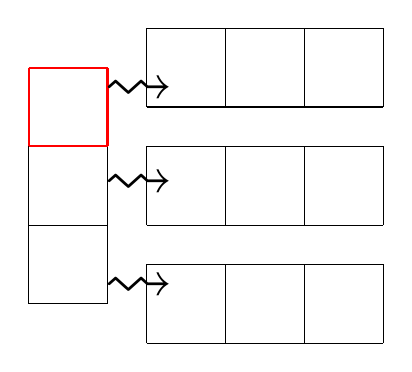
\begin{tikzpicture}

\draw grid(1,3);
\draw [xshift=1.5cm, yshift=2.5cm]grid(3,1);
\uncover<3>{\draw [red, thick, xshift=0cm, yshift=2cm]grid(1,1);}
\draw [xshift=1.5cm, yshift=1cm]grid(3,1);
\draw [xshift=1.5cm, yshift=-.5cm]grid(3,1);
\node at (1.4, 1.5) {\Huge $\rightsquigarrow$};   
\node at (1.4, 2.7) {\Huge $\rightsquigarrow$};   
\node at (1.4, 0.2) {\Huge $\rightsquigarrow$};   

\end{tikzpicture}
\end{adjustbox}

}
\end{minipage} 
}

\uncover<4-6>{
\vspace{-5em}
The first, in memory:
\begin{align*}
\uncover<6>{\m{arraddr} (\m{ptr}, \m{i},\texttt{size}) \defeq~&
  \m{ptr} + (\m{i} \times \hide{\texttt{sizeof}(\texttt{int}) \times} \texttt{size}) \\ }
\uncover<5->{\p{rowrep}(\gamma, \m{i}, \m{ptr}) \defeq~& \texttt{let }\m{row} \texttt{ := }\mathsf{graph2mat}(\gamma)[\m{i}] \texttt{ in } \\ 
&\mathsf{array}(\mathit{arraddr}(\m{ptr},\m{i},\lvert\m{row}\rvert), \m{row}) \\ }
\vspace{1em}
\p{AdjMat}(\gamma, \m{gaddr}, \_) \defeq~& \underset{\m{v}\hspace{0.1em}\in \gamma}{\bigstar} \p{rowrep}(\gamma, \m{v}, \m{gaddr})
\end{align*}
}

\end{frame}


\section{Shortest Path: Dijkstra}

\begin{frame}[fragile]{Dijkstra: \texttt{SoundDijk}}
\begin{lstlisting}
Class SoundDijk size inf g := {
  sadjmat: SoundAdjMat size inf g;
  efr: $\forall$e, evalid g e $\rightarrow$
           0 $\le$ elabel g e $\le$ $\alert<2>{\texttt{(MAX/size)}}$;
  ifr: $\alert<3>{\texttt{(MAX/(size-1)) * size}}$ $<$ inf 
}.
\end{lstlisting}

{\centering
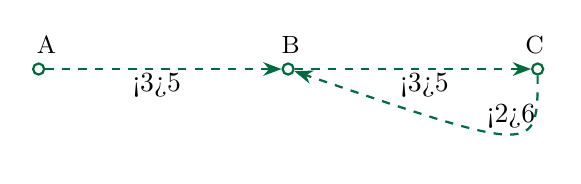
\begin{tikzpicture}
[inf/.style={circle, draw=myred, thick, inner sep=0pt, minimum size=4pt},
 ->/.style={thick, arrows={-Stealth}}]

  \node at (1.5,-0.2) {\alert<3>5};
  \node at (4.9,-0.2) {\alert<3>5};
  \node at (6,-0.6) {\alert<2>6};
 
\node at (0.1, 0.3) {\small A};
\node at (3.2, 0.3) {\small B};
\node at (6.3, 0.3) {\small C}; 
  \node[inf] (A) at (0,0) {};
  \node[inf] (B) [right = 3 of A] {};
  \node[inf] (C) [right = 3 of B] {};
 
  \draw [->, dashed, myred] (A) -- (B);
  \draw [->, dashed, myred] (B) -- (C);
  \draw [->, dashed, myred] (C.south) .. controls ++(0, -1) .. (B);
\end{tikzpicture}
  
 }
 
 \uncover<2->{\hspace{1.8em}\texttt{efr: }Leave room for probing link} \\
 \uncover<3>{\hspace{1.8em}\texttt{ifr: }Bona-fide costs must dodge \texttt{inf}} 


\end{frame} 

\begin{frame}{Dijkstra: spatial representation}
Nothing fancy spatially, use \p{AdjMat} wholesale \\
We verify Dijkstra 3 times: \\
\hspace{1em} reuse math proof entirely \\
\hspace{1em} spatial variations handled under the hood

\end{frame}

\begin{frame}[fragile]{Dijkstra: code and specification}

\begin{lstlisting}
void dijkstra (int **g, int src, int *dist, 
               int *prev, int size, int inf {
 /* elided: init PQ, fill out dist and prev */
 while (size(pq)) {
\end{lstlisting}
\pause
$\braces{{\exists \m{dist}, \m{prev}, \m{popped}}.~ 
\m{dijk\_correct}(\gamma,\texttt{src},\m{popped},\m{prev},\m{dist})}$
\end{frame}

\begin{frame}{Dijkstra: intuition for \m{dijk\_correct}}

\begin{center}
\begin{adjustbox}{scale=0.50}
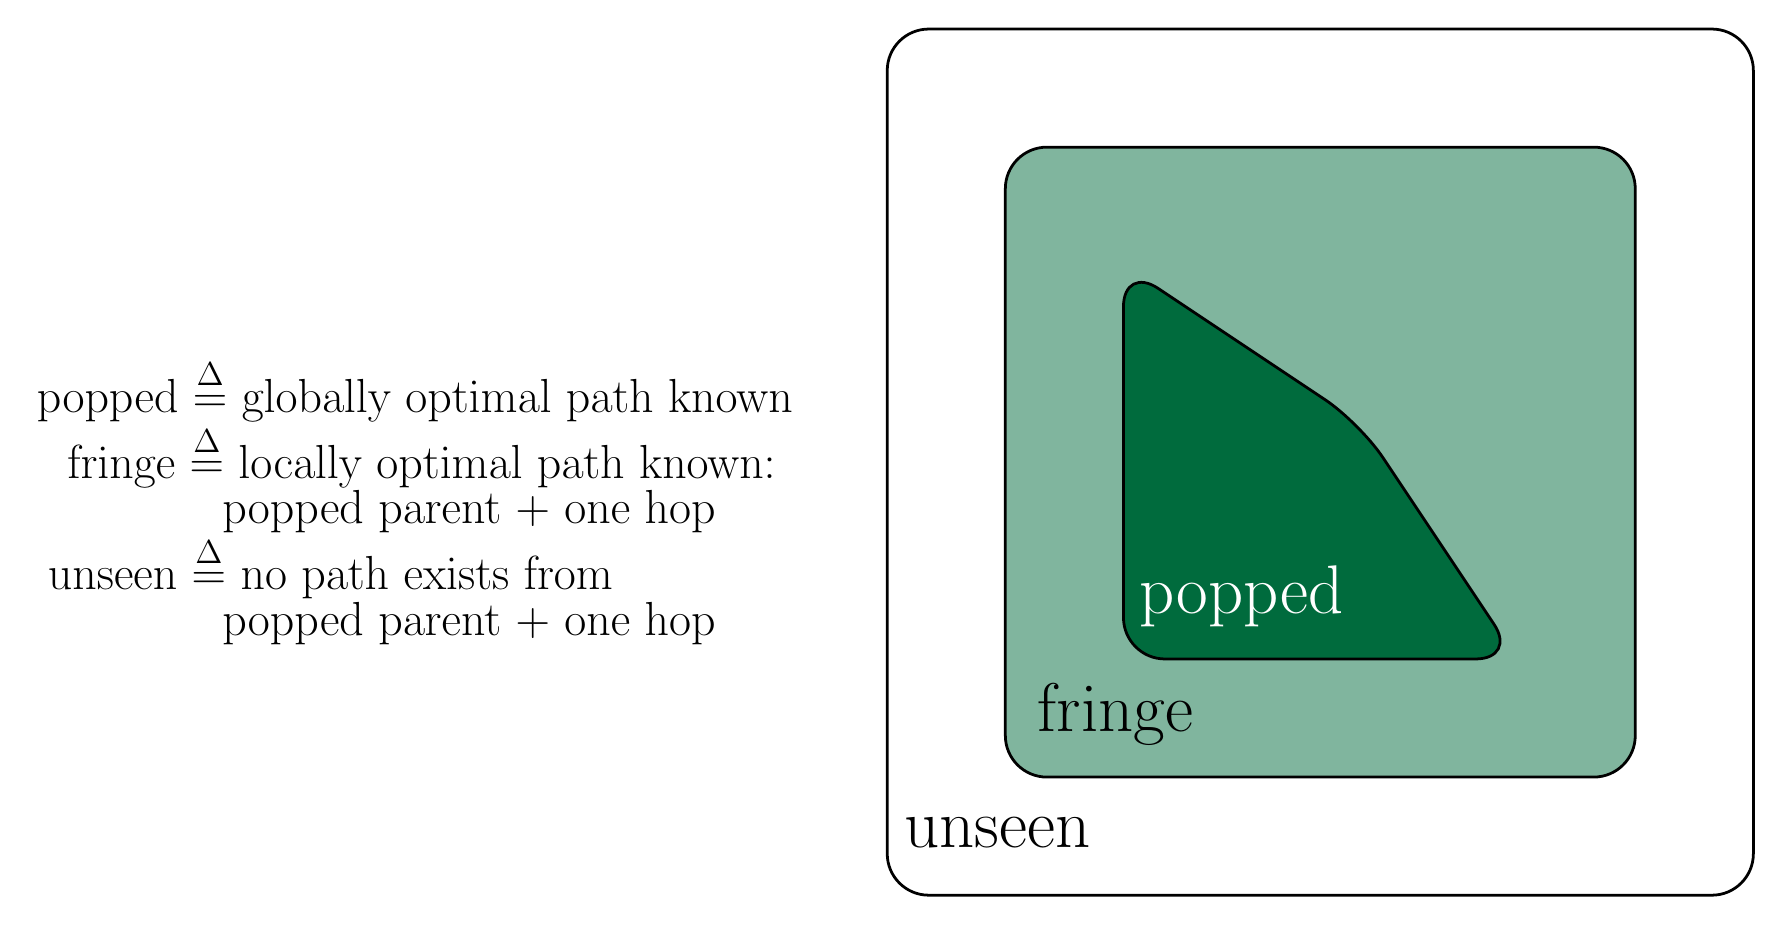
\begin{tikzpicture}[on grid,
  popped/.style={rounded corners=15pt, line width=1pt, draw, fill=myred},
  fringe/.style={rounded corners=15pt, line width=1pt, draw, fill=mypink},
  popping/.style={rounded corners=15pt, line width=1pt, draw, dashed, fill=mymaroon},
  unseen/.style={rounded corners=15pt, line width=1pt, draw},
   every text node part/.style={align=left}]

  \uncover<1>{
  \draw[unseen] (0,0) -- (\s,0) -- (\s,\s) -- (0,\s) -- cycle;
  \draw[fringe] (1.5,1.5) -- (9.5,1.5) -- (9.5,9.5) -- (1.5,9.5) -- cycle;
  \draw[popped] (3,3) -- (8,3) -- (6,6) -- (3,8) -- cycle;
  \node at (1.4,0.8) {\Huge unseen};   
  \node at (2.9,2.3) {\Huge fringe};   
  \node at (4.5,3.8) {\Huge \color{white}popped};
  \node at (-6,5) {\LARGE popped $\defeq$ globally optimal path known \\
  \hspace{1.1em}\LARGE fringe $\defeq$ locally optimal path known: \\
  \hspace{6.7em}\LARGE popped parent + one hop \\
  \hspace{0.4em}\LARGE unseen $\defeq$ no path exists from \\
  \hspace{6.7em}\LARGE popped parent + one hop}; }  

  \end{tikzpicture}
\end{adjustbox}
\end{center}
\end{frame}


\begin{frame}[fragile]{Dijkstra: code and specification}
\begin{lstlisting}
 while (size(pq)) {
\end{lstlisting}
$\braces{\m{dijk\_correct}(\gamma,\texttt{src},\m{popped},\m{prev},\m{dist})}$
\pause
\begin{lstlisting}
  u = popMin(pq);
\end{lstlisting}
\pause
\begin{lstlisting}
  for (i = 0; i < size; i++) {
\end{lstlisting}
$\braces{\exists \m{dist'}, \m{prev'}~
\m{dijk\_correct\_weak}(\gamma, \texttt{src}, \m{popped} \uplus \{\texttt{u}\}, \m{prev'}, \m{dist'}, \texttt{i}, \texttt{u})}$

\end{frame}

\begin{frame}{Dijkstra: intuition for \m{dijk\_correct\_weak}}

\begin{center}
\begin{adjustbox}{scale=0.50}
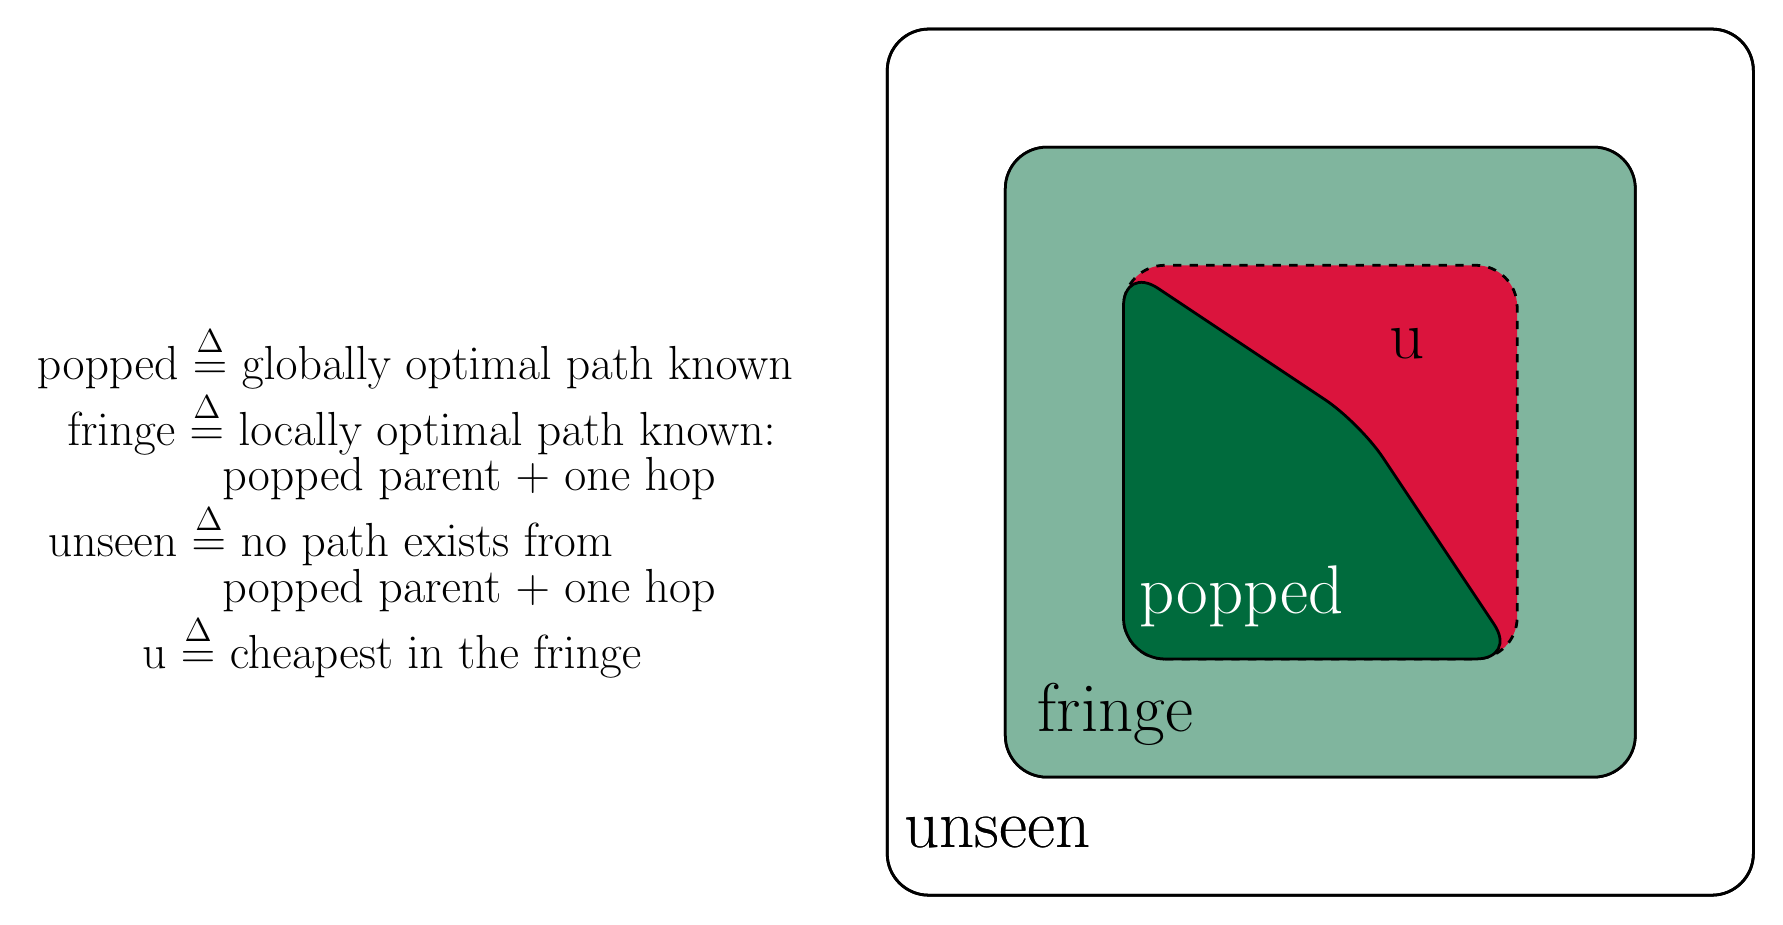
\begin{tikzpicture}[on grid,
  popped/.style={rounded corners=15pt, line width=1pt, draw, fill=myred},
  fringe/.style={rounded corners=15pt, line width=1pt, draw, fill=mypink},
  popping/.style={rounded corners=15pt, line width=1pt, draw, dashed, fill=mymaroon},
  unseen/.style={rounded corners=15pt, line width=1pt, draw},
  every text node part/.style={align=left}]
  \uncover<1>{
  \draw[unseen] (0,0) -- (\s,0) -- (\s,\s) -- (0,\s) -- cycle;
  \draw[fringe] (1.5,1.5) -- (9.5,1.5) -- (9.5,9.5) -- (1.5,9.5) -- cycle;
  \draw[popped] (3,3) -- (8,3) -- (6,6) -- (3,8) -- cycle;
  \node at (1.4,0.8) {\Huge unseen};   
  \node at (2.9,2.3) {\Huge fringe};   
  \node at (4.5,3.8) {\Huge \color{white}popped};
  \node at (6.6,7) {\Huge u};}
\uncover<1->{  
\node at (-6,5) {\LARGE popped $\defeq$ globally optimal path known \\
  \hspace{1.1em}\LARGE fringe $\defeq$ locally optimal path known: \\
  \hspace{6.7em}\LARGE popped parent + one hop \\
  \hspace{0.4em}\LARGE unseen $\defeq$ no path exists from \\
  \hspace{6.7em}\LARGE popped parent + one hop \\
  \hspace{3.8em}\LARGE u $\defeq$ cheapest in the fringe}; }  
  \uncover<2>{
    \draw[unseen] (0,0) -- (\s,0) -- (\s,\s) -- (0,\s) -- cycle;
  \draw[fringe] (1.5,1.5) -- (9.5,1.5) -- (9.5,9.5) -- (1.5,9.5) -- cycle;
  \draw[popping] (3,3) -- (8,3) -- (8,8) -- (3,8) -- cycle;
  \draw[popped] (3,3) -- (8,3) -- (6,6) -- (3,8) -- cycle;
  \node at (1.4,0.8) {\Huge unseen};   
  \node at (2.9,2.3) {\Huge fringe};   
  \node at (4.5,3.8) {\Huge \color{white}popped};
  \node at (6.6,7) {\Huge u}; }
\end{tikzpicture}
\end{adjustbox}
\end{center}
\end{frame}

\begin{frame}[fragile]{Dijkstra: code and specification}
\begin{lstlisting}
 while (size(pq)) {
\end{lstlisting}
$\braces{\m{dijk\_correct}(\gamma,\texttt{src},\m{popped},\m{prev},\m{dist})}$
\begin{lstlisting}
  u = popMin(pq);
  for (i = 0; i < size; i++) {
\end{lstlisting}
$\color{OliveGreen}\braces{{\exists \m{dist'}, \m{prev'}}.~
{\m{dijk\_correct\_weak}(\gamma, \texttt{src}, \m{popped} \uplus \{\texttt{u}\}, \m{prev'}, \m{dist'}, \texttt{i}, \texttt{u})}}$
\pause
\begin{lstlisting}
  /* elided: potentially relax edge (u,i) */
 }} /* for */  
\end{lstlisting}

\end{frame}

\begin{frame}{Dijkstra: intuition for recovering \m{dijk\_correct}}

\begin{center}
\begin{adjustbox}{scale=0.50}
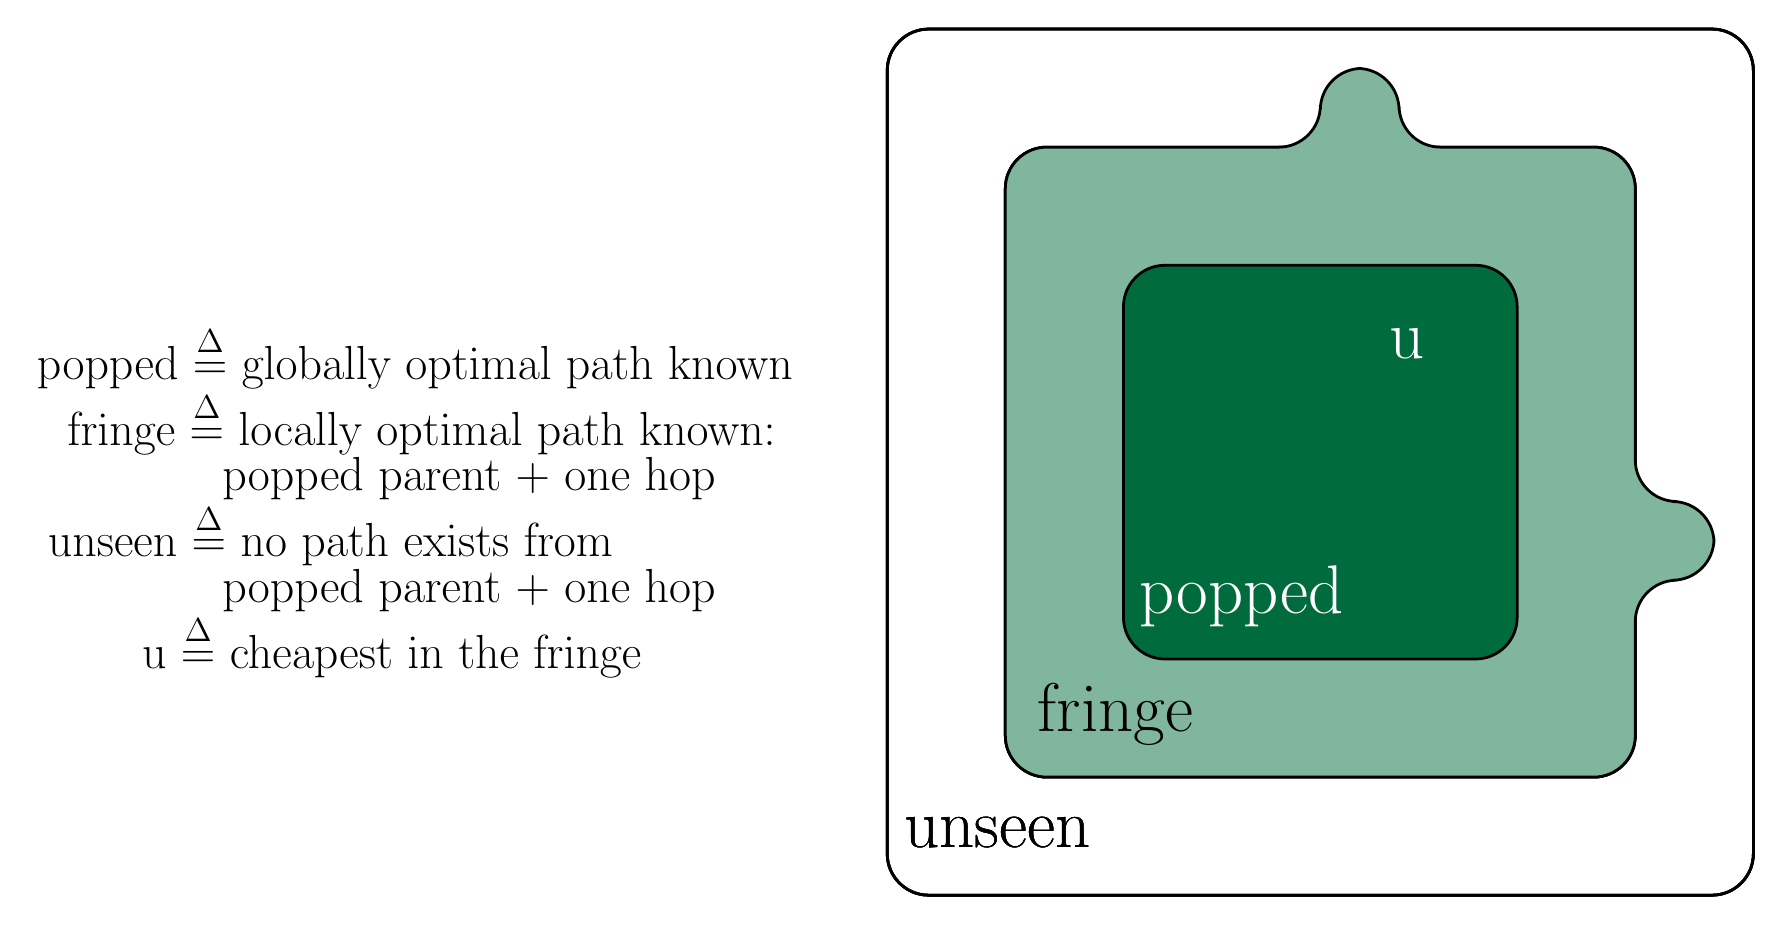
\begin{tikzpicture}[on grid,
  popped/.style={rounded corners=15pt, line width=1pt, draw, fill=myred},
  fringe/.style={rounded corners=15pt, line width=1pt, draw, fill=mypink},
  popping/.style={rounded corners=15pt, line width=1pt, draw, dashed, fill=mymaroon},
  unseen/.style={rounded corners=15pt, line width=1pt, draw},
  every text node part/.style={align=left}]

  \uncover<1>{
  \draw[unseen] (0,0) -- (\s,0) -- (\s,\s) -- (0,\s) -- cycle;
  \draw[fringe] (1.5,1.5) -- (9.5,1.5) -- (9.5,9.5) -- (1.5,9.5) -- cycle;
  \draw[popped] (3,3) -- (8,3) -- (6,6) -- (3,8) -- cycle;
  \node at (1.4,0.8) {\Huge unseen};   
  \node at (2.9,2.3) {\Huge fringe};   
  \node at (4.5,3.8) {\Huge \color{white}popped};
  \node at (6.6,7) {\Huge u};}
  \uncover<1->{   
  \node at (-6,5) {\LARGE popped $\defeq$ globally optimal path known \\
  \hspace{1.1em}\LARGE fringe $\defeq$ locally optimal path known: \\
  \hspace{6.7em}\LARGE popped parent + one hop \\
  \hspace{0.4em}\LARGE unseen $\defeq$ no path exists from \\
  \hspace{6.7em}\LARGE popped parent + one hop \\ 
  \hspace{3.8em}\LARGE u $\defeq$ cheapest in the fringe}; }  

  \uncover<2>{
    \draw[unseen] (0,0) -- (\s,0) -- (\s,\s) -- (0,\s) -- cycle;
  \draw[fringe] (1.5,1.5) -- (9.5,1.5) -- (9.5,9.5) -- (1.5,9.5) -- cycle;
  \draw[popping] (3,3) -- (8,3) -- (8,8) -- (3,8) -- cycle;
  \draw[popped] (3,3) -- (8,3) -- (6,6) -- (3,8) -- cycle;
  \node at (1.4,0.8) {\Huge unseen};   
  \node at (2.9,2.3) {\Huge fringe};   
  \node at (4.5,3.8) {\Huge \color{white}popped};
  \node at (6.6,7) {\Huge u}; }
  \uncover<3>{
    \draw[unseen] (0,0) -- (\s,0) -- (\s,\s) -- (0,\s) -- cycle;
  \draw[fringe] (1.5,1.5) -- (9.5,1.5) -- (9.5, 4.0) -- (10.5, 4.0) -- (10.5, 5.0) -- (9.5, 5.0) -- (9.5,9.5) -- (6.5, 9.5) -- (6.5, 10.5) -- (5.5, 10.5) -- (5.5, 9.5) -- (1.5,9.5) -- cycle;
  \draw[popped] (3,3) -- (8,3) -- (8,8) -- (3,8) -- cycle;
  \node at (1.4,0.8) {\Huge unseen};   
  \node at (2.9,2.3) {\Huge fringe};   
  \node at (4.5,3.8) {\Huge \color{white}popped};
  \node at (6.6,7) {\Huge \color{white}u}; }
\end{tikzpicture}
\end{adjustbox}
\end{center}
\end{frame}

\begin{frame}[fragile]{Dijkstra: code and specification}
\begin{lstlisting}
 while (size(pq)) {
\end{lstlisting}
$\braces{\m{dijk\_correct}(\gamma,\texttt{src},\m{popped},\m{prev},\m{dist})}$
\begin{lstlisting}
  u = popMin(pq);
  for (i = 0; i < size; i++) {
\end{lstlisting}
$\color{OliveGreen}\braces{{\exists \m{dist'}, \m{prev'}}.~
{\m{dijk\_correct\_weak}(\gamma, \texttt{src}, \m{popped} \uplus \{\texttt{u}\}, \m{prev'}, \m{dist'}, \texttt{i}, \texttt{u})}}$
\begin{lstlisting}
  /* elided: potentially relax edge (u,i) */
 }} /* for */  
\end{lstlisting}
\pause
\vspace{-2.3em}
\begin{lstlisting}
                 } /* while */
\end{lstlisting}
\pause
$\braces{\exists \m{dist''}, \m{prev''}.~
\forall \m{dst}.~0 \le \m{dst} < \texttt{size} \rightarrow \null \\ 
\m{inv\_popped}(\gamma, \m{src}, \m{\gamma.V}, \m{prev''}, \m{dist''}, \m{dst})}$
\begin{lstlisting}
 freePQ (pq); return;  } /* func */
\end{lstlisting}

\end{frame}

\hide{
\begin{frame}{dijk\_correct\_weak}

\begin{equation*}
\begin{split}
&\hspace{-1em}\m{dijk\_correct\_weak}(\gamma, \m{src}, \m{popped}, \m{prev}, \m{dist}, \m{i}, \m{u}) \; \defeq \; \forall \m{d}.~ \\
&\alert<2>{\big( vvalid(\gamma, \m{d}) \; \Rightarrow} \; \m{d} \in \m{popped} \; \Rightarrow \; \ldots \alert<2>{\big)} \wedge \\
&\alert<2>{\Big( 0 \le dst < i \; \Rightarrow} \; 
\big( \m{dist}[\m{d}] < \ifty \; \Rightarrow \ldots \big) \wedge
\big( \m{dist}[\m{d}] = \ifty \; \Rightarrow \ldots \big) \alert<2>{\Big)} \wedge \null \\
&\alert<3>{\Big( i \le dst < size \; \Rightarrow} \; \null \\
&\hspace{1em}\big( \m{dist}[\m{d}] < \ifty \; \Rightarrow \ldots \alert<4>{\wedge m \neq u \wedge m' \neq u} \big) \wedge \null \\
&\hspace{1em}\big( \m{dist}[\m{d}] = \ifty \; \Rightarrow \ldots \alert<4>{\wedge m \neq u} \big) \alert<3>{\Big)} \\
\end{split}
\end{equation*}

\end{frame}
} % end hide

\begin{frame}{Dijkstra: postcondition}

\begin{center}
\begin{adjustbox}{scale=0.50}
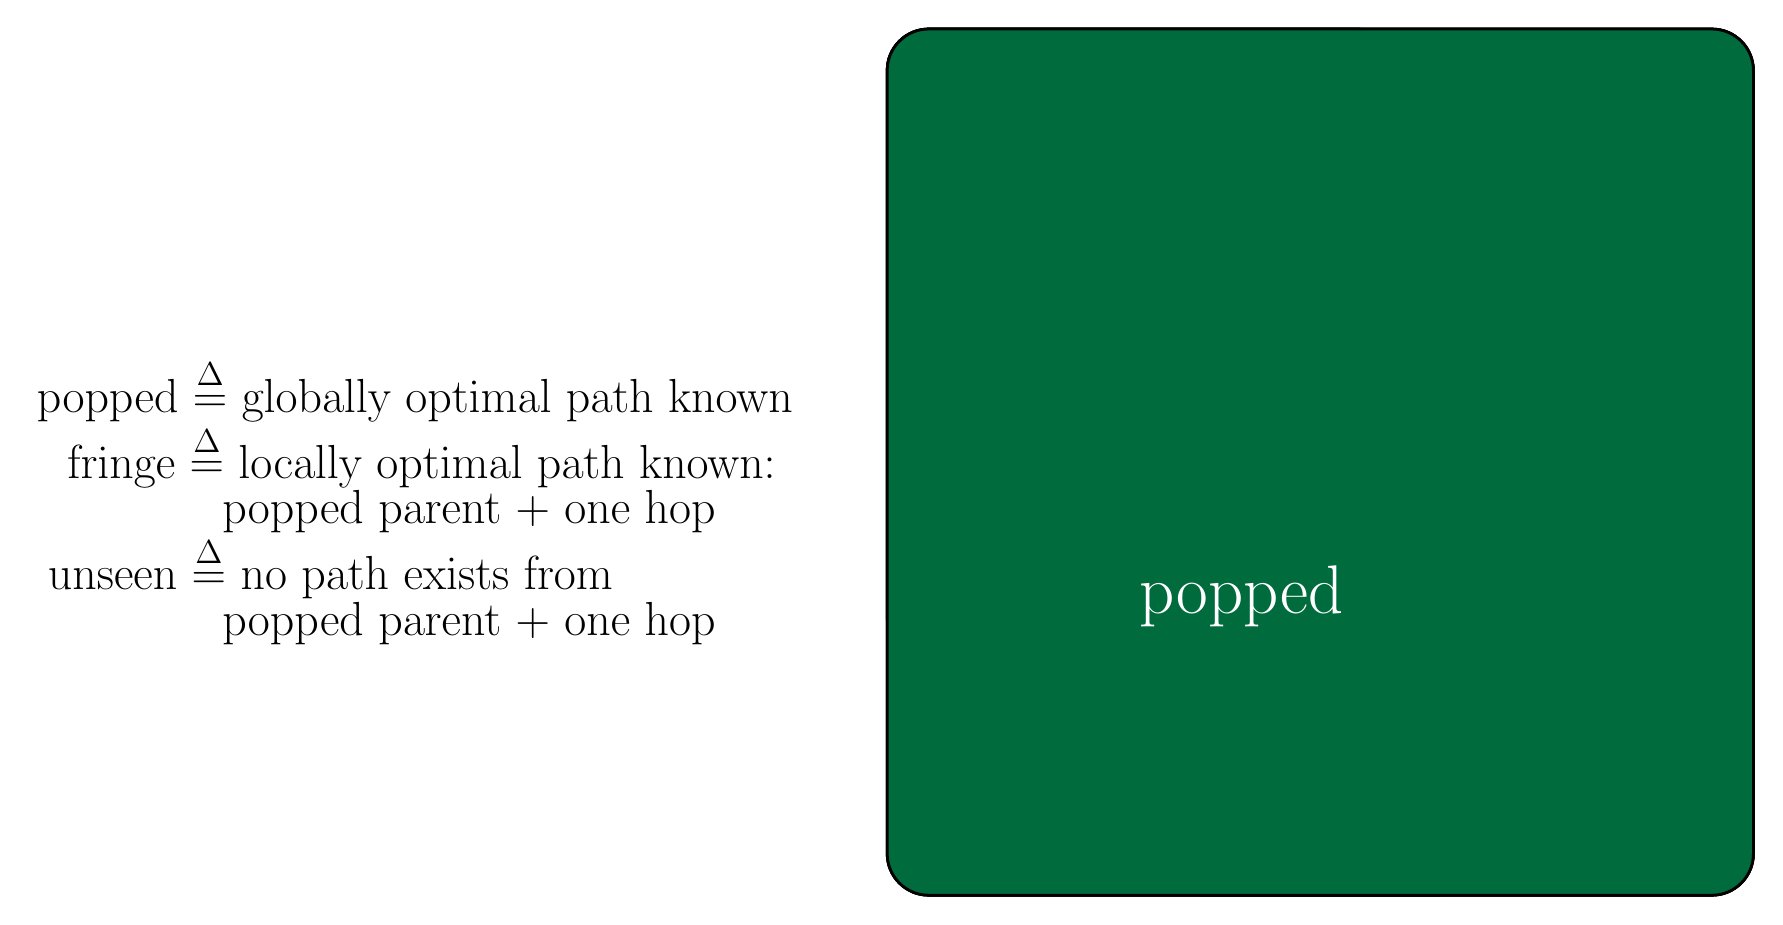
\begin{tikzpicture}[on grid,
  popped/.style={rounded corners=15pt, line width=1pt, draw, fill=myred},
  fringe/.style={rounded corners=15pt, line width=1pt, draw, fill=mypink},
  popping/.style={rounded corners=15pt, line width=1pt, draw, dashed, fill=mymaroon},
  unseen/.style={rounded corners=15pt, line width=1pt, draw},
  every text node part/.style={align=left}]
  
  \uncover<1>{
    \draw[unseen] (0,0) -- (\s,0) -- (\s,\s) -- (0,\s) -- cycle;
  \draw[fringe] (1.5,1.5) -- (9.5,1.5) -- (9.5, 4.0) -- (10.5, 4.0) -- (10.5, 5.0) -- (9.5, 5.0) -- (9.5,9.5) -- (6.5, 9.5) -- (6.5, 10.5) -- (5.5, 10.5) -- (5.5, 9.5) -- (1.5,9.5) -- cycle;
  \draw[popped] (3,3) -- (8,3) -- (8,8) -- (3,8) -- cycle;
  \node at (1.4,0.8) {\Huge unseen};   
  \node at (2.9,2.3) {\Huge fringe};   
  \node at (4.5,3.8) {\Huge \color{white}popped};}
  \uncover<1->{  
  \node at (-6,5) {\LARGE popped $\defeq$ globally optimal path known \\
  \hspace{1.1em}\LARGE fringe $\defeq$ locally optimal path known: \\
  \hspace{6.7em}\LARGE popped parent + one hop \\
  \hspace{0.4em}\LARGE unseen $\defeq$ no path exists from \\
  \hspace{6.7em}\LARGE popped parent + one hop}; }  

  \uncover<2>{
    \draw[fringe] (0,0) -- (\s,0) -- (\s,\s) -- (0,\s) -- cycle;
  \draw[popped] (1.5,1.5) -- (3.5, 1.5) -- (3.5, 0) -- (7.5, 0) -- (7.5, 1.5) -- (9.5,1.5) -- (9.5, 4.0) -- (11, 4.0) -- (11, 8.0) -- (9.5, 8.0) -- (9.5,9.5) -- (6.5, 9.5) -- (6.5, 11) -- (0, 11) -- (0, 3) -- (1.5, 3) -- cycle;
  \node at (4.5,3.8) {\Huge \color{white}popped}; 
  \node at (1.5,.8) {\Huge fringe}; } 

  \uncover<3>{
    \draw[popped] (0,0) -- (\s,0) -- (\s,\s) -- (0,\s) -- cycle;
  \node at (4.5,3.8) {\Huge \color{white}popped}; }
  
\end{tikzpicture}
\end{adjustbox}
\end{center}
\end{frame}

\section{Undirectedness in a Directed World}

\begin{frame}[fragile]{Undirectedness in a directed world}

CertiGraph is fundamentally directed \\
We layer undirectedness atop of this

\pause \bigskip

\hspace{1em} Build lightweight undirected definitions \\
\hspace{1em} Prove connections to existing directed definitions \\
\hspace{1em} Grow undirected infrastructure

\end{frame}

\begin{frame}{Weakening directed into undirected}

\m{x} and \m{y} are $\texttt{adjacent}^{u}$ if there is an $\texttt{edge}^{d}$ between them: \\
\hspace{1em} \m{x} $\rightarrow$ \m{y} or \m{y} $\rightarrow$ \m{x} \\

\pause \bigskip

$\texttt{connected}^{u}$ is the transitive closure of $\texttt{adjacent}^{u}$: \\
\hspace{1em} \m{x} $\rightsquigarrow$ \m{a} $\leftarrow$ \m{b} $\leftarrow$ \m{c} $\leftsquigarrow$ \m{y} \\

\pause \bigskip

We already have $\texttt{reachable}^{d}$: \hspace{0.5em} \m{x} $\rightsquigarrow$ \m{y} \\
\pause
By design, $\texttt{reachable}^{d}$ weakens easily into $\texttt{connected}^{u}$

\pause \bigskip

$\texttt{connected}^{u}$ is powerful enough to define \\
$\texttt{cycle}^{u}$, $\texttt{forest}^{u}$, $\texttt{spanning}^{u}$, $\ldots$ ,
$\texttt{minimum\_spanning\_forest}^{u}$

\end{frame}

\hide{
\begin{frame}[fragile]{Building an undirected infrastructure}

A \texttt{upath} is the edge-sequence connecting two \texttt{connected} vertices \\
A \texttt{ucycle} is a \texttt{upath} with \m{head} = \m{foot} \\
\texttt{is\_partial\_graph f g} means that everything in \texttt{f} is also in \texttt{g}
\bigskip \pause
\begin{lstlisting}
Definition uforest g := $\forall$ p l, $\lnot$ucycle g p l.

Definition spanning g g' :=
 $\forall$ u v, connected g u v $\leftrightarrow$ connected g' u v.

Definition spanning_uforest f g :=
  is_partial_graph f g $\wedge$ uforest f $\wedge$ spanning f g.
\end{lstlisting}

\bigskip \pause
And \texttt{minimum\_spanning\_forest f g} means that \\
\texttt{f} minimizes total edge cost among other \texttt{spanning\_uforest}s of \texttt{g}

\end{frame}
} % end hide

\begin{frame}[fragile]{\texttt{SoundUAdjMat}, the undirected soundness condition}

\begin{minipage}{0.45\textwidth}
{\centering
\begin{adjustbox}{scale=0.8}
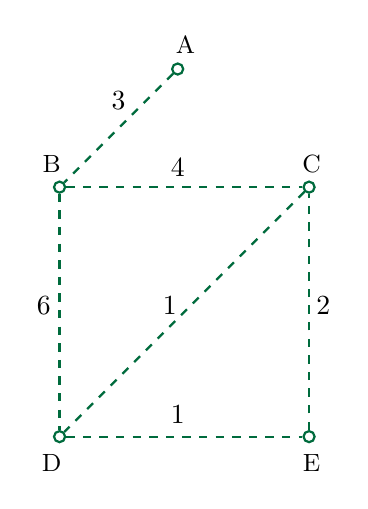
\begin{tikzpicture}
[vad/.style={rectangle, fill=black, inner sep=0pt, minimum size=4pt},
 inf/.style={circle, draw=myred, thick, inner sep=0pt, minimum size=4pt},
 inv/.style={circle, fill=myred, draw=myred, thick, inner sep=0pt, minimum size=4pt},
 ->/.style={thick, arrows={-Stealth}},
 every text node part/.style={align=center}]
 
% static vertices and their labels
\node at (1.6, 1.8) {\small A};
\node at (-0.1, 0.3) {\small B};
\node at (3.2, 0.3) {\small C};
\node at (-0.1, -3.5) {\small D}; 
\node at (3.2, -3.5) {\small E}; 
\node[inf] (A) at (1.5,1.5) {};  
\node[inf] (B) at (0,0) {};
\node[inf] (C) [right = 3 of B] {};
\node[inf] (D) [below = 3 of B] {};
\node[inf] (E) [below = 3 of C] {};

\node at (.75,1.1) {3};
\node at (1.5,0.25) {4};
\node at (1.5,-2.89) {1};
\node at (-0.2,-1.5) {6};
\node at (3.35,-1.5) {2};
\node at (1.4,-1.5) {1};

  \draw [thick, dashed, myred] (A) -- (B);
  \draw [thick, dashed, myred] (B) -- (C);
  \draw [thick, dashed, myred] (D) -- (E);  
  \draw [thick, dashed, myred] (B) -- (D);
  \draw [thick, dashed, myred] (E) -- (C);
  \draw [thick, dashed, myred] (C) -- (D);
 
\end{tikzpicture}
\end{adjustbox}

}
\end{minipage} \begin{minipage}{0.45\textwidth}
{\centering
\begin{adjustbox}{scale=0.8}
\tikz\draw grid(5,5)foreach[count=~]\l in 
{  , A, B, C, D, E,
 A, $\infty$, 3, $\infty$, $\infty$, $\infty$,
 B, 3, $\infty$, 4, 6, $\infty$,
 C, $\infty$, 4, $\infty$, 1, 2,
 D, $\infty$, 6, 1, $\infty$, 1, 
 E, $\infty$, $\infty$, 2, 1, $\infty$}
{({-.5+mod(~-1,6},{5.5-div(~-1,6})node{\l}};
\end{adjustbox}

}
\end{minipage}

\bigskip \pause

A little trick prevents double-counting:

\begin{lstlisting}
Class SoundUAdjMat size inf g := {
  sadjmat: SoundAdjMat size inf g;
  undirec: $\forall$e, evalid g e $\rightarrow$ src g e $\le$ dst g e;
}.
\end{lstlisting}

\end{frame}

\begin{frame}[fragile]{\texttt{SoundUAdjMat}, the undirected soundness condition}

\begin{minipage}{0.45\textwidth}
{\centering
\begin{adjustbox}{scale=0.8}
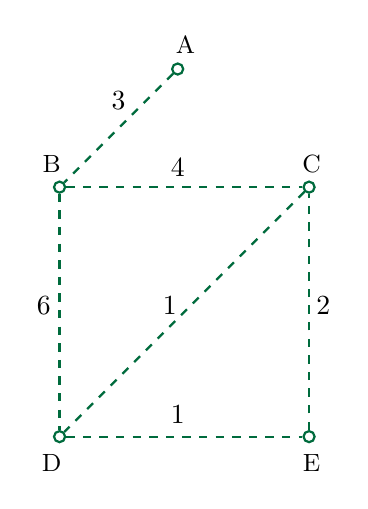
\begin{tikzpicture}
[vad/.style={rectangle, fill=black, inner sep=0pt, minimum size=4pt},
 inf/.style={circle, draw=myred, thick, inner sep=0pt, minimum size=4pt},
 inv/.style={circle, fill=myred, draw=myred, thick, inner sep=0pt, minimum size=4pt},
 ->/.style={thick, arrows={-Stealth}},
 every text node part/.style={align=center}]
 
% static vertices and their labels
\node at (1.6, 1.8) {\small A};
\node at (-0.1, 0.3) {\small B};
\node at (3.2, 0.3) {\small C};
\node at (-0.1, -3.5) {\small D}; 
\node at (3.2, -3.5) {\small E}; 
\node[inf] (A) at (1.5,1.5) {};  
\node[inf] (B) at (0,0) {};
\node[inf] (C) [right = 3 of B] {};
\node[inf] (D) [below = 3 of B] {};
\node[inf] (E) [below = 3 of C] {};

\node at (.75,1.1) {3};
\node at (1.5,0.25) {4};
\node at (1.5,-2.89) {1};
\node at (-0.2,-1.5) {6};
\node at (3.35,-1.5) {2};
\node at (1.4,-1.5) {1};

  \draw [thick, dashed, myred] (A) -- (B);
  \draw [thick, dashed, myred] (B) -- (C);
  \draw [thick, dashed, myred] (D) -- (E);  
  \draw [thick, dashed, myred] (B) -- (D);
  \draw [thick, dashed, myred] (E) -- (C);
  \draw [thick, dashed, myred] (C) -- (D);
 
\end{tikzpicture}
\end{adjustbox}

}
\end{minipage} \begin{minipage}{0.45\textwidth}
{\centering
\begin{adjustbox}{scale=0.8}
\tikz\draw grid(5,5)foreach[count=~]\l in 
{  , A, B, C, D, E,
 A, $\infty$, 3, $\infty$, $\infty$, $\infty$,
 B, $\alert{\infty}$, $\infty$, 4, 6, $\infty$,
 C, $\alert{\infty}$, $\alert{\infty}$, $\infty$, 1, 2,
 D, $\alert{\infty}$, $\alert{\infty}$, $\alert{\infty}$, $\infty$, 1, 
 E, $\alert{\infty}$, $\alert{\infty}$, $\alert{\infty}$, $\alert{\infty}$, $\infty$}
{({-.5+mod(~-1,6},{5.5-div(~-1,6})node{\l}};
\end{adjustbox}

}
\end{minipage}

\bigskip

A little trick prevents double-counting:

\begin{lstlisting}
Class SoundUAdjMat size inf g := {
  sadjmat: SoundAdjMat size inf g;
  undirec: $\forall$e, evalid g e $\rightarrow$ $\alert{\m{fst} \texttt{ e} \le \m{snd} \texttt{ e}}$;
}.
\end{lstlisting}

\end{frame}

\section{Minimum Spanning Forest: Prim and Kruskal}

\begin{frame}[fragile]{Prim: missing the forest for the trees}

\begin{minipage}{0.60\textwidth}
\begin{lstlisting}
MST-PRIM(G,w,r):
 for each u in G.V
  /* elided: set up PQ, 
     key, parent */
 r.key = 0
 while PQ $\neq$ $\emptyset$
  u = EXTRACT-MIN(PQ) 
  for each v in G.Adj[u]
   if (v $\in$ Q and 
       w(u,v) $<$ v.key)
    v.parent = u
    v.key = w(u,v) $\hide{code:primeditpri}$
\end{lstlisting} 

\bigskip \pause
\uncover<2-3>{
Prim typically assumes a connected graph}
\end{minipage} \begin{minipage}{0.35\textwidth}
\uncover<2->{
{\centering
\begin{adjustbox}{scale=0.8}
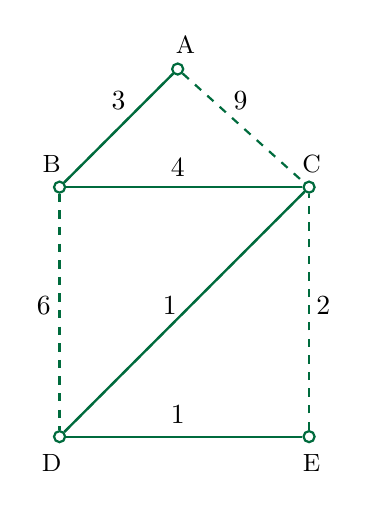
\begin{tikzpicture}
[vad/.style={rectangle, fill=black, inner sep=0pt, minimum size=4pt},
 inf/.style={circle, draw=myred, thick, inner sep=0pt, minimum size=4pt},
 inv/.style={circle, fill=myred, draw=myred, thick, inner sep=0pt, minimum size=4pt},
 ->/.style={thick, arrows={-Stealth}},
 every text node part/.style={align=center}]
 
% static vertices and their labels
\node at (1.6, 1.8) {\small A};
\node at (-0.1, 0.3) {\small B};
\node at (3.2, 0.3) {\small C};
\node at (-0.1, -3.5) {\small D}; 
\node at (3.2, -3.5) {\small E}; 
\node[inf] (A) at (1.5,1.5) {};  
\node[inf] (B) at (0,0) {};
\node[inf] (C) [right = 3 of B] {};
\node[inf] (D) [below = 3 of B] {};
\node[inf] (E) [below = 3 of C] {};

\node at (.75,1.1) {3};
\node at (1.5,0.25) {4};
\node at (1.5,-2.89) {1};
\node at (1.4,-1.5) {1};
\uncover<2>{\node at (2.3,1.1) {9};
		    \node at (-0.2,-1.5) {6};
	             \node at (3.35,-1.5) {2};
			}

 \uncover<2>{
  \draw [thick, dashed, myred] (B) -- (A);
  \draw [thick, dashed, myred] (C) -- (B);
  \draw [thick, dashed, myred] (E) -- (D);
  \draw [thick, dashed, myred] (C) -- (D);
   \draw [thick, dashed, myred] (B) -- (D);
  \draw [thick, dashed, myred] (E) -- (C);
  \draw [thick, dashed, myred] (A) -- (C);
  }
  \uncover<3>{
  \draw [thick, myred] (B) -- (A);
  \draw [thick, myred] (C) -- (B);
  \draw [thick, myred] (E) -- (D);
  \draw [thick, myred] (C) -- (D);
 }

\end{tikzpicture}
\end{adjustbox}

}}
\end{minipage}

\end{frame}

\begin{frame}[fragile]{Prim: missing the forest for the trees}

\begin{minipage}{0.60\textwidth}
\begin{lstlisting}
MST-PRIM(G,w,r):
 for each u in G.V
  /* elided: set up PQ, 
     key, parent */
 r.key = 0
 while PQ $\neq$ $\emptyset$
  $\alert<4->{\texttt{u = EXTRACT-MIN(PQ)}}$ 
  for each v in G.Adj[u]
   if (v $\in$ Q and 
       w(u,v) $<$ v.key)
    v.parent = u
    v.key = w(u,v) $\hide{code:primeditpri}$
\end{lstlisting} 

\bigskip \vspace{-1em}
How about an unconnected graph? \\
\uncover<4->{D can now be extracted at cost \texttt{inf} \\ } 
\uncover<5->{\hspace{-.35em}meaning D is the root of a new tree 
\includegraphics[scale=.08]{nye}}
\end{minipage} \begin{minipage}{0.35\textwidth}
\uncover<2->{
{\centering
\begin{adjustbox}{scale=0.9}
\begin{tikzpicture}
[vad/.style={rectangle, fill=black, inner sep=0pt, minimum size=4pt},
 inf/.style={circle, draw=myred, thick, inner sep=0pt, minimum size=4pt},
 inv/.style={circle, fill=myred, draw=myred, thick, inner sep=0pt, minimum size=4pt},
 ->/.style={thick, arrows={-Stealth}},
 every text node part/.style={align=center}]
 
% static vertices and their labels
\node at (1.6, 1.8) {\small A};
\node at (-0.1, 0.3) {\small B};
\node at (3.2, 0.3) {\small C};
\node at (-0.1, -3.5) {\small D}; 
\node at (3.2, -3.5) {\small E}; 
\node[inf] (A) at (1.5,1.5) {};  
\node[inf] (B) at (0,0) {};
\node[inf] (C) [right = 3 of B] {};
\node[inf] (D) [below = 3 of B] {};
\node[inf] (E) [below = 3 of C] {};

%edge labels 
\node at (.75,1.1) {3};
\node at (1.5,0.25) {4};
\node at (1.5,-2.89) {1};
\uncover<2>{\node at (2.3,1.1) {9};}
 
 %undirected
 \uncover<2->{
  \draw [thick, dashed, myred] (B) -- (A);
  \draw [thick, dashed, myred] (C) -- (B);
  \draw [thick, dashed, myred] (E) -- (D);
  }
  \uncover<2>{
  \draw [thick, dashed, myred] (A) -- (C);
 }
 \uncover<3->{\draw [thick, myred] (B) -- (A);}
 \uncover<3->{\draw [thick, myred] (C) -- (B);}
 \uncover<6>{\draw [thick, myred] (E) -- (D);}

 
\end{tikzpicture}
\end{adjustbox}

}}
\end{minipage}

\end{frame}


\begin{frame}[fragile]{Prim: an unnecessary argument; a simpler spec}

\begin{minipage}{0.48\textwidth}
\begin{lstlisting}
MST-PRIM(G,w,$\alert{\texttt{r}}$):
 for each u in G.V
  u.key = INF
  u.parent = NIL $\hide{code:primsetinitparent}$
 $\alert{\texttt{r.key = 0}}$
 Q = G.V
 while Q $\neq$ $\emptyset$
  u = EXTRACT-MIN(Q) $\hide{code:primextractmin}$
  for each v in G.Adj[u]
   if (v $\in$ Q and 
       w(u,v) $<$ v.key)
    v.parent = u
    v.key = w(u,v) $\hide{code:primeditpri}$
\end{lstlisting} \end{minipage}
\begin{minipage}{0.5\textwidth}
\begin{lstlisting}
MST-PRIM-NOROOT(G,w):
 for each u in G.V
  u.key = INF
  u.parent = NIL $\hide{code:primsetinitparent}$

 Q = G.V
 while Q $\neq$ $\emptyset$
  u = EXTRACT-MIN(Q) $\hide{code:primextractmin}$
  for each v in G.Adj[u]
   if (v $\in$ Q and 
       w(u,v) $<$ v.key)
    v.parent = u
    v.key = w(u,v) $\hide{code:primeditpri}$
\end{lstlisting} 
\end{minipage} 
\end{frame}


\begin{frame}{Kruskal: challenges and nonchallenges}
Extend spatial support: \\
\hspace{1em} lay out edgelist-represented graphs in memory \\
\hspace{1em} develop fold-unfold utilities in separation logic

\bigskip

The undirected development carries over wholesale

\bigskip

Manipulate two graphs simultaneously: \\
\hspace{1em}directed graph with vertex labels (stores parents and ranks) \\
\hspace{1em}undirected graph with edge labels (for which we construct an MSF)
\end{frame}

\begin{frame}{Kruksal: layering undirectedness atop of union-find}
  We have just performed $\texttt{union}^{d}$ \m{a} \m{b} \\
  \vspace{2em}
  {\centering
  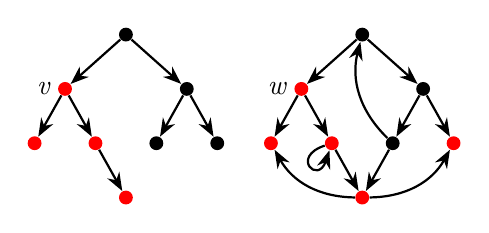
\begin{tikzpicture}[
  gnode/.style={circle, inner sep=0pt, minimum size=5pt, fill=black},
  gnodecol/.style={circle, inner sep=0pt, minimum size=5pt, fill=red},
  ->/.style={-Stealth, thick}, node distance=0.5cm]
  \node[gnode] (n0) {};
  \node[gnodecol] (n1) [below = of n0, xshift=-22pt] {};
  \node [left = of n1, xshift = 16pt] {$\m{v}$};
  \node[gnode] (n2) [below = of n0, xshift=22pt] {};
  \node[gnodecol] (n3) [below = of n1, xshift=-11pt] {};
  \node[gnodecol] (n4) [below = of n1, xshift=11pt] {};
  \node[gnode] (n5) [below = of n2, xshift=-11pt] {};
  \node[gnode] (n6) [below = of n2, xshift=11pt] {};
  \node[gnodecol] (n7) [below = of n4, xshift=11pt] {};
  \draw[->] (n0) to (n1);
  \draw[->] (n0) to (n2);
  \draw[->] (n1) to (n3);
  \draw[->] (n1) to (n4);
  \draw[->] (n2) to (n5);
  \draw[->] (n2) to (n6);
  \draw[->] (n4) to (n7);
  \node[gnode] (m0) [right = 80pt of n0]{};
  \node[gnodecol] (m1) [below = of m0, xshift=-22pt] {};
  \node [left = of m1, xshift = 16pt] {$\m{w}$};
  \node[gnode] (m2) [below = of m0, xshift=22pt] {};
  \node[gnodecol] (m3) [below = of m1, xshift=-11pt] {};
  \node[gnodecol] (m4) [below = of m1, xshift=11pt] {};
  \node[gnode] (m5) [below = of m2, xshift=-11pt] {};
  \node[gnodecol] (m6) [below = of m2, xshift=11pt] {};
  \node[gnodecol] (m7) [below = of m4, xshift=11pt] {};
  \draw[->] (m0) to (m1);
  \draw[->] (m0) to (m2);
  \draw[->] (m1) to (m3);
  \draw[->] (m1) to (m4);
  \draw[->] (m2) to (m5);
  \draw[->] (m2) to (m6);
  \draw[->] (m4) to (m7);
  \draw[->] (m5) to (m7);
  \draw[->] (m5) to [bend left] (m0);
  \draw[->] (m4) .. controls ([xshift=-15pt, yshift=-5pt] m4) and ([xshift=-5pt, yshift=-15pt] m4) .. (m4);
  \draw[->] (m7) to [bend right] (m6);
  \draw[->] (m7) to [bend left] (m3);
\end{tikzpicture}

  
  }
 \pause \bigskip
  What can we say about $\texttt{connected}^{u}$ \m{a} \m{b}? \uncover<3>{$\texttt{connected}^{u}$ \m{c} \m{b}?}
\end{frame}

\begin{frame}{Contributions}
\uncover<1->{
Math, spatial support for adjacency matrices, edge lists \\
Harmonious math support for undirected graphs \\ }
\bigskip
\uncover<2->{
Dijkstra: nontrivial overflow \\ }
\uncover<3->{
Prim: nontrivial improvement in spec \\ }
\uncover<4->{
Kruskal: library handles directed $+$ undirected \\ }
\bigskip
\uncover<5->{
Development is modular and general \\
High effort---largely because we work with C---but good reuse}
\bigskip
\uncover<6->{
\flushright
Thanks! \hspace{2em}}
\end{frame}

\end{document}
